\section{Introduction}
In contemporary radiation therapy, photon intensity modulated radiation therapy (IMRT) stands as a pivotal technique utilized to attain precise and conformal dose distributions within target volumes \cite{xu_comparison_2017}.
This achievement owes its realization chiefly to the advent of the multileaf collimator (MLC) \cite{galvin_characterization_1993}.

Radiation therapy is now a reliable treatment for oncology \cite{valentini_survival_2009}.
Despite this consensus, the way to deliver radiotherapy for its best result remain very dependent upon doctors.
Moreover, it appears that there is a large variability across physicians and centers, bot in terms of 3D structures contouring and irradiation constraints priorities \cite{variability_2021}.

To achieve the best treatment, doctors need to solve a complex inverse mathematical optimization problem with multiples trade-offs \cite{oelfke_inverse_2001} \cite{webb_physical_2003}.
There is a lack of standardized prioritization of constraints make the optimization a real challenge.
The standard procedure nowadays is to manually guide computer optimization: dosimetrists manually update the settings of an optimizing software (so called Treatment Planning System) \cite{planification_website}.

There has been many tries to create a metric that quantify the quality of a treatment plan: Normal tissue complication probabilities (NTCP), Target coverage, Conformity index, Heterogeneity index (non-exhaustive list) \cite{lyman_normal_1992} \cite{li_input_2022}.\label{metrics}
However, none of them has been able to satisfy all radio-oncologists, and the only reliable way of assessing a plan for doctors is to check out the dose-volume histograms (DVHs) them-self.

As a result, Pareto surface exploration are doomed to failure due to the lack of impartial quantitative measurement for a particular plan \cite{huang_pareto_2021}.
Other meta-optimization techniques are similarly bounded, for the same reason \cite{wu_optimization_2001} \cite{xing_optimization_1999}.
An extra challenge to attend for those is the fact that not all cases have the same "difficulty".
Hence, for an "easy" case, doctors will require an excellent dose (in terms of the metrics mentioned above), while they can be more permissive for "harder" cases.
This make the acceptability of a plan hard to define in general.

Reinforcement learning is a machine learning paradigm concerned with training agents to make sequential decisions in dynamic environments \cite{brooks_what_2021}.
Through a process of trial and error guided by rewards or penalties, agents learn to optimize their actions to achieve long-term objectives.
It appears that the decisions taken by dosimetrists when performing the optimization of a treatment can be formalized as a reinforcement learning problem.
Moreover, dosimetrists can guide the TPS towards an acceptable plan, but they usually struggle explaining their decision while interacting with the TPS.
This suggest the use of deep reinforcement learning, over expert base methods.

\section{Materials and Methods}
We introduce a new paradigm in reinforcement learning (RL), based on the evaluation of states, rather than the reward.

\subsection{Reinforcement Learning Reward}

\begin{figure*}
	\centering
	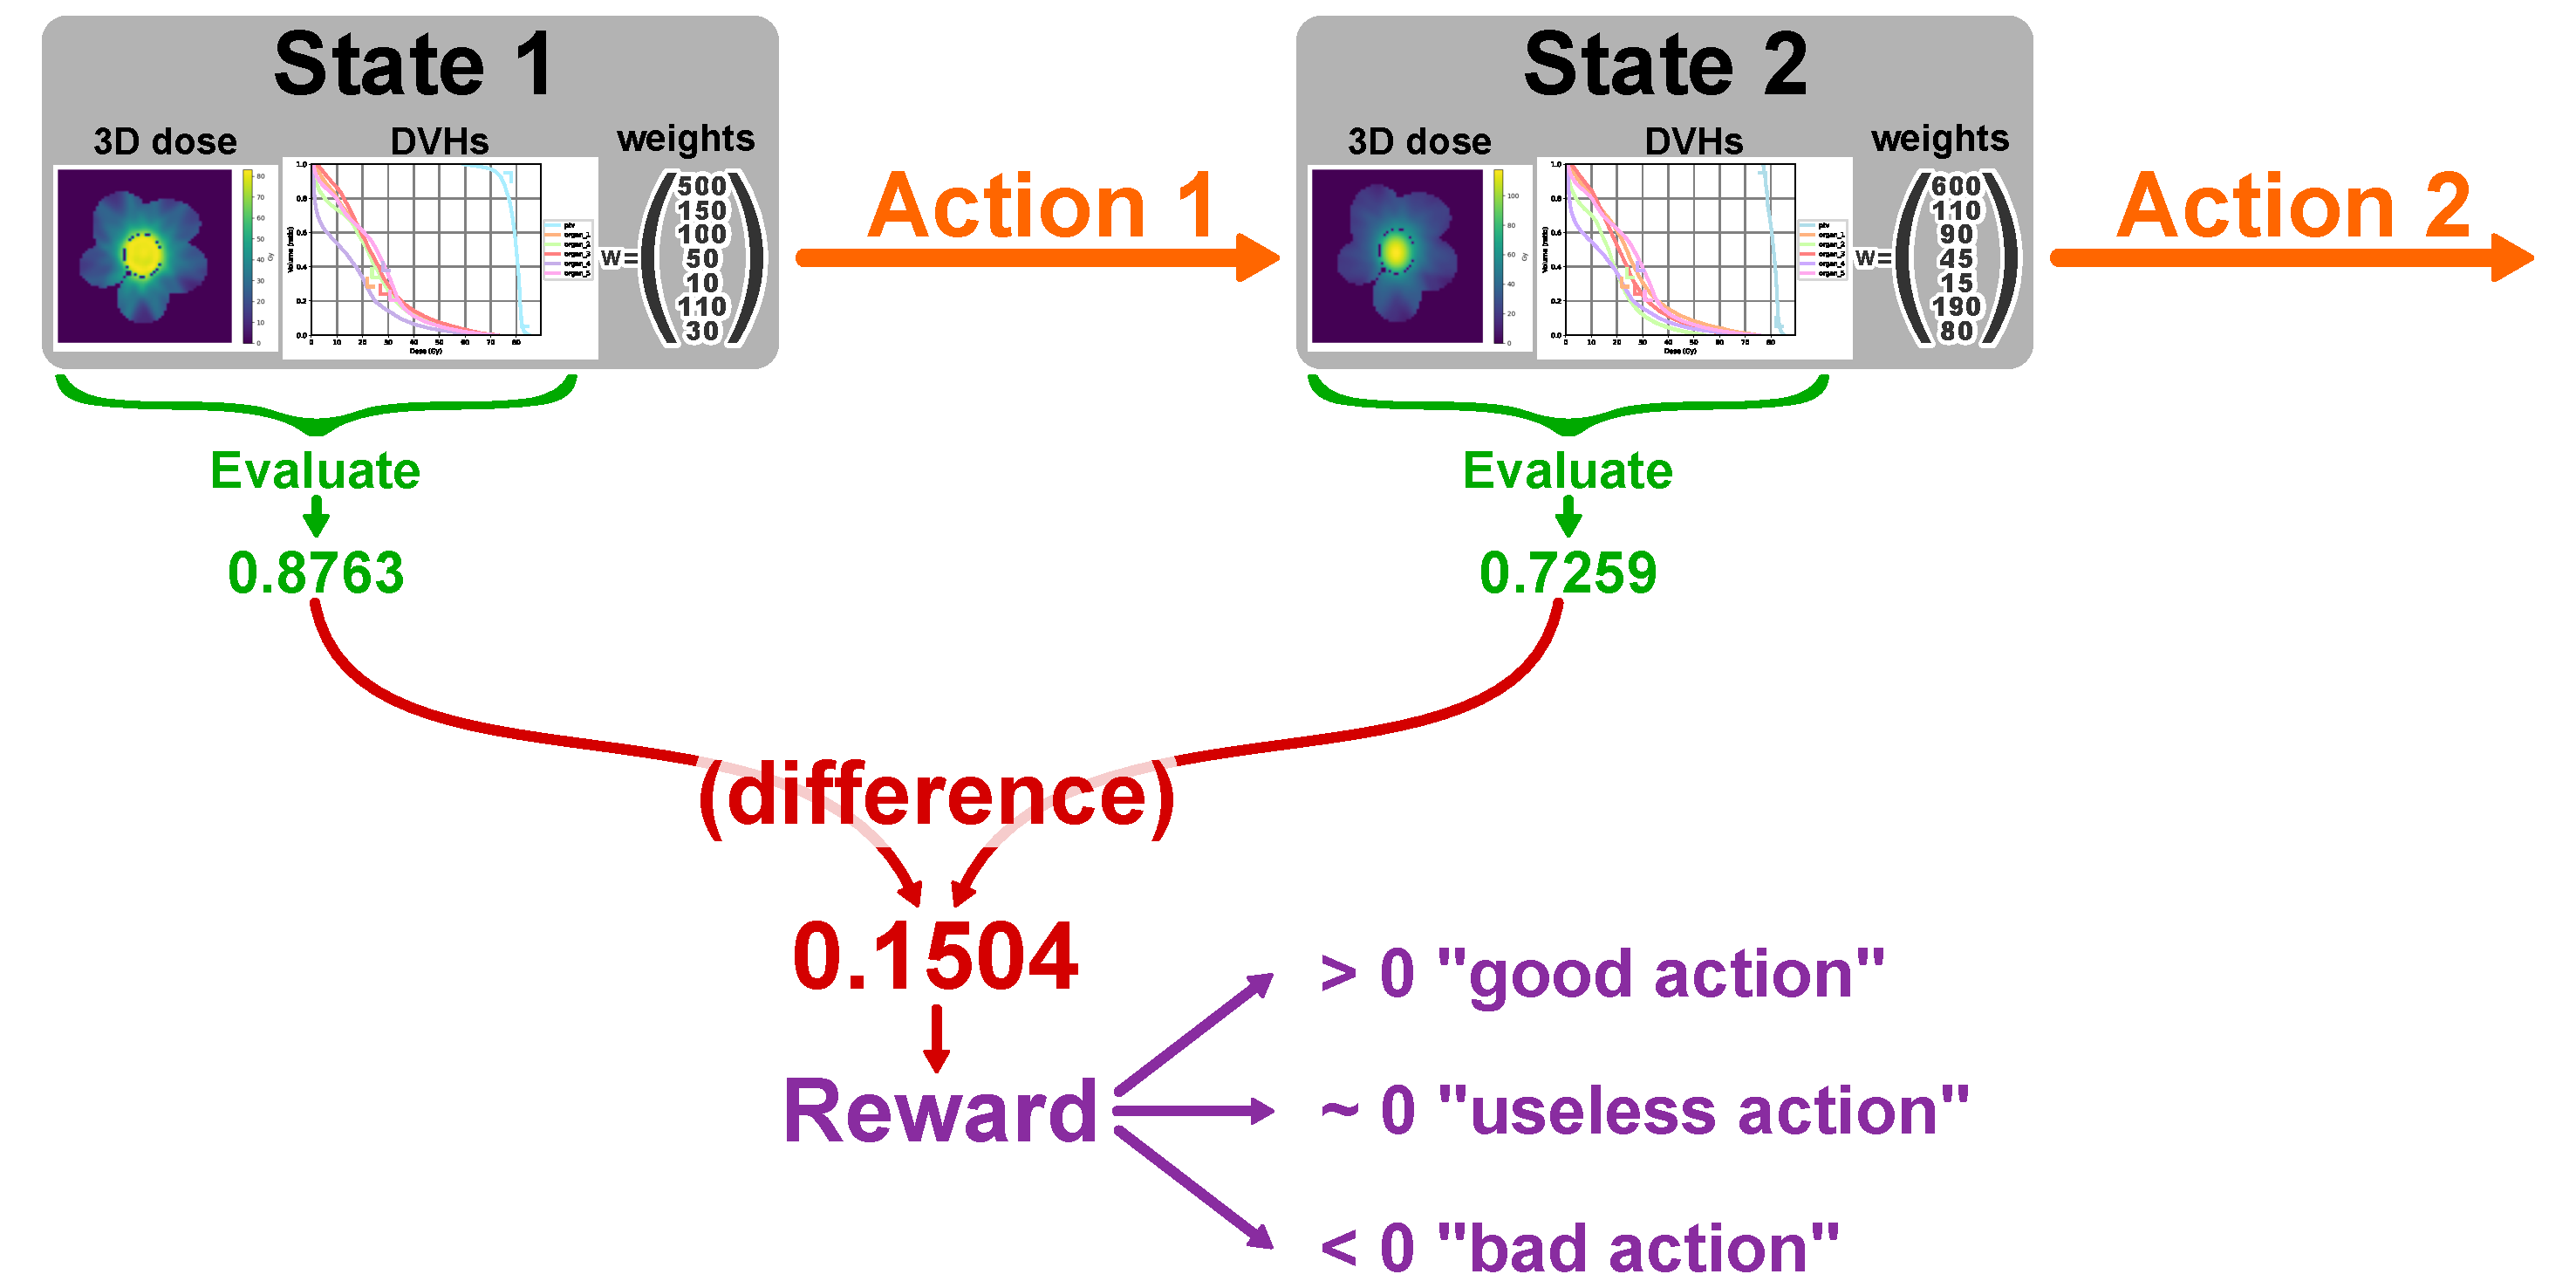
\includegraphics[width=0.8\textwidth]{reward.pdf}
	\caption{Classical reinforcement learning reward for automatic dosimetry.}
	\label{fig:reward_fig}
\end{figure*}

In classical RL, we want $V(S_t) = R_t + \gamma V(S_{t+1})$
(so the update is $V(S_t) \leftarrow (1-\alpha) V(S_t) + \alpha \left[ R_{t+1} + \gamma V(S_{t+1}) \right]$).
In the context of dose optimization, the reward $R_t$ is defined as $R_t = \mathcal{E}(S_{t+1}) - \mathcal{E}(S_t)$.
Where $\mathcal{E}$ is a function that evaluates the quality of a state (such that higher is better; if lower is better, then swap $s_t$ and $S_{t+1}$).

The evaluation $\mathcal{E}$ can be one, or a mixture of the metrics mentions in introduction (Section \ref{metrics}) \cite{shen_hierarchical_2021} \cite{shen_intelligent_2019} \cite{moreau_reinforcement_2021}.
This setup may leverage knowledge about which actions to perform, instead of guessing randomly as a meta optimizer would do.
We can hope to gain some computation time.

However, this technique is not using the plan used in past cases; it only needs the optimizer inputs (CT, structures contours).
We propose to use the availability of past treatment plans, to better catch the complexity of decision taken by dosimetrists, and match better their expectations of a fully automatic treatment planning system.

As developed in previous work, we can derive a distance between doses plans [add citation].
If we consider the clinical dose of past cases (used for training) as the best achievable one, then we can evaluate a dose plan by computing its distance with the clinical dose plan.

Letting $D_t$ be the dose associated with $S_t$, and $D_C$ the clinical dose.
We then define $\mathcal{E}(S_t) = \mathcal{D}(D_t, D_C)$.
Since in that case, lower is better, we will define the reward as $$R_t = \mathcal{E}(S_t) - \mathcal{E}(S_{t+1}) = \mathcal{D}(D_t, D_C) - \mathcal{D}(D_{t+1}, D_C).$$
This reward can be interpreted as the "distance gained to the clinical dose".


\subsection{Reward-Free Reinforcement Learning}

Since the reward is based on an evaluation of the state, one may consider dropping all the reward machinery, and directly use the state evaluation.
This allows us to better capture the signal: it is not embedded in a reward system, and the network can therefore learn faster.

The reason why reward system is used in many games (such as go or chess) is that state evaluation is extremely difficult, if not impossible; there is no function that, given the board, gives the quality of white/black's position.
Reward is only given at the end of a game, usually $+1$ for winning, $-1$ for losing.
The states evaluation are deduced by the reinforcement learning agent while learning to maximize the reward.

However, in our dosimetrist case, we exactly have such an evaluation function.
Embedding this evaluation in a reward, by defining the reward as the evaluation difference turns out to dilute the signal, and the agent learns slower.

By predicting the next state evaluation instead of using the Bellman optimality equation, we lose the ability to make short term concessions in order to obtain reward later on.
In our case, making short term concessions would mean that we trigger the weights in a way that the optimizer performs worse, but such that triggering a little more makes the optimizer perform better.

Because optimizers have the bad habit od getting stuck in local minimum, we can not use last optimization result as a "warm start" after modifying optimization weights.
Hence, restarting optimization from zero is forced after every weight modification.

Given the statement of the optimization problem, and the fact that we can not use warm start, making short term compromises does not make much sense.
It is therefore safe to predict next state evaluation directly, without the use of the Bellman optimality equation.

\subsection{Avoiding Over-fitting}
We use a dense neural network, taking the DVHs and the currents normalized weights values as inputs.
Dense layers are very prone to over fitting.
In order to force the network to actually predict the next evaluation for each possible action, without over-fitting, we incorporated a bottle neck in the network.
Compressing the information stops the network from learning "by heart".
Networks with such architecture show significantly better results on validation.
%This comfort the idea that our network was learning from data, without blindly over-fitting.

\subsection{Avoiding Off-Distribution}
We generated a training set of over 125k actions (this took 5 days on an NVIDIA GeForce GTX 1080).
Despite this relatively large dataset, we have not explored exhaustively the state-actions space, and the network still gets off distribution.
This can easily be spotted when the predicted distance is negative; we choose to ignore those predictions.
In fact, we ignore all outliers prediction.
The justification is that our set of action is limited, there is no action that will suddenly drastically improve the plan.
It is the combination of several sequential actions that allows good plan optimization.
Therefore, while testing, we choose the action with best prediction, while passing the outlier test just mentioned.

\section{Results}

\section{Discussion}


\section*{Appendix}

\subsection*{Synthetic phantom patients}
As this is very new and ongoing research, we generated synthetic phantom patients and associated trust-able clinical dose.
In future work, we hope to be able to apply this technique to real cases.

\subsection*{Clinical dose}

\subsection*{Optimization}

\subsection*{Evaluation}

